\scanpage{159}
\figure{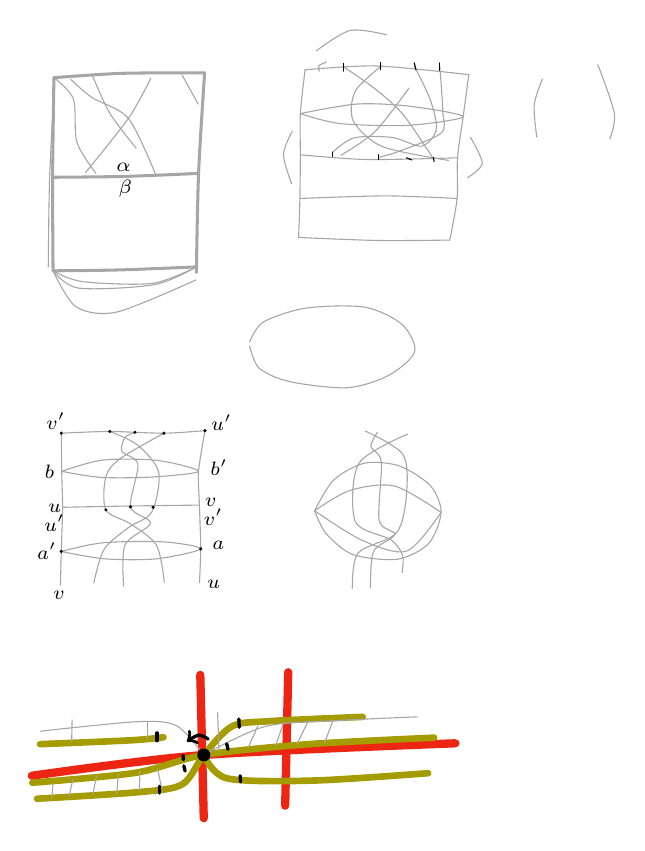
\begin{tikzpicture}[x=.55cm,y=-.55cm,line cap=round,line join=round,g/.style={olive!80!yellow,line width=1.7pt},r/.style={orange!80!brown,line width=1.8pt},w/.style={red!60!black,line width=1.5pt},b/.style={blue!60!black,line width=1.4pt},p/.style={gray!70,thin},k/.style={black,line width=1.2pt},every node/.style={font=\scriptsize}]
\draw[p,line width=1.1pt] plot[smooth] coordinates {(2.71,2.67) (4.29,2.57) (6.19,2.56)};
\draw[p,line width=1.1pt] plot[smooth] coordinates {(2.71,2.67) (2.68,4.97) (2.69,7.13)};
\draw[p,line width=1.1pt] plot[smooth] coordinates {(6.19,2.56) (6.05,4.88) (6.0,7.17)};
\draw[p,line width=1.1pt] plot[smooth] coordinates {(2.68,4.97) (4.36,4.95) (6.05,4.88)};
\draw[p,line width=1.1pt] plot[smooth] coordinates {(2.69,7.13) (4.2,7.11) (6.0,7.04)};
\draw[p] plot[smooth] coordinates {(2.71,2.67) (3.16,3.16) (3.24,4.16) (3.68,4.88)};
\draw[p] plot[smooth] coordinates {(3.1,2.71) (3.59,3.13) (4.43,3.61) (5.06,4.91)};
\draw[p] plot[smooth] coordinates {(3.59,2.6) (4.0,3.49) (4.61,4.3)};
\draw[p] plot[smooth] coordinates {(4.95,2.68) (4.43,3.61) (3.44,4.86)};
\draw[p] plot[smooth] coordinates {(5.67,2.61) (6.04,3.28)};
\draw[p] plot[smooth] coordinates {(2.69,7.13) (3.37,7.38) (4.98,7.42) (6.0,7.04)};
\draw[p] plot[smooth] coordinates {(2.69,7.13) (3.28,7.53) (5.03,7.45) (6.0,7.04)};
\draw[p] plot[smooth] coordinates {(2.69,7.13) (3.22,7.96) (4.17,8.08) (5.99,7.34)};
\draw[p] plot[smooth] coordinates {(2.72,2.8) (2.61,5.0) (2.58,7.04)};
\node at (4.32,4.74) {$\alpha$};
\node at (4.36,5.24) {$\beta$};
\draw[p] plot[smooth] coordinates {(8.51,2.49) (10.15,2.4) (12.29,2.6)};
\draw[p] plot[smooth] coordinates {(8.51,2.49) (8.4,3.5) (8.4,4.45) (8.39,5.46) (8.36,6.36)};
\draw[p] plot[smooth] coordinates {(12.29,2.6) (12.16,3.57) (12.03,4.52) (12.02,5.46) (11.85,6.42)};
\draw[p] plot[smooth] coordinates {(8.4,3.5) (9.7,3.28) (10.93,3.33) (12.16,3.57) (10.9,3.77) (9.32,3.73) (8.4,3.5)};
\draw[p] plot[smooth] coordinates {(8.4,4.45) (9.93,4.56) (12.03,4.52)};
\draw[p] plot[smooth] coordinates {(8.39,5.46) (10.37,5.4) (12.02,5.46)};
\draw[p] plot[smooth] coordinates {(8.36,6.36) (10.2,6.43) (11.85,6.42)};
\draw[p] plot[smooth] coordinates {(8.21,3.91) (8.01,4.45) (8.2,5.12)};
\draw[p] plot[smooth] coordinates {(12.33,4.05) (12.6,4.65) (12.26,4.98)};
\draw[p] plot[smooth] coordinates {(8.84,2.52) (8.83,2.39) (9.01,2.31)};
\draw[p] plot[smooth] coordinates {(9.4,2.42) (10.14,2.94) (10.78,3.53) (11.47,4.54)};
\draw[p] plot[smooth] coordinates {(10.26,2.41) (9.67,2.98) (9.62,3.66) (10.29,4.26) (11.82,4.58)};
\draw[p] plot[smooth] coordinates {(11.03,2.4) (11.4,3.18) (11.54,3.87) (11.2,4.25) (10.52,4.05) (9.64,4.06) (9.15,4.39)};
\draw[p] plot[smooth] coordinates {(11.62,2.4) (11.69,3.45) (11.65,3.95) (10.68,4.37) (10.21,4.51)};
\draw[p] plot[smooth] coordinates {(9.34,4.46) (10.13,3.91) (10.91,2.91)};
\draw[p] plot[smooth] coordinates {(13.99,2.7) (13.8,3.3) (13.86,4.04)};
\draw[p] plot[smooth] coordinates {(15.27,2.37) (15.65,3.49) (15.55,4.08)};
\draw[p] plot[smooth] coordinates {(8.77,2.05) (9.55,1.58) (10.39,1.68)};
\draw[k,thin] plot[smooth] coordinates {(9.4,2.34) (9.4,2.52)};
\draw[k,thin] plot[smooth] coordinates {(10.26,2.32) (10.26,2.49)};
\draw[k,thin] plot[smooth] coordinates {(11.03,2.33) (11.07,2.49)};
\draw[k,thin] plot[smooth] coordinates {(11.62,2.33) (11.62,2.5)};
\draw[k,thin] plot[smooth] coordinates {(9.15,4.39) (9.15,4.49)};
\draw[k,thin] plot[smooth] coordinates {(10.21,4.45) (10.21,4.56)};
\draw[k,thin] plot[smooth] coordinates {(10.85,4.52) (10.97,4.57)};
\draw[k,thin] plot[smooth] coordinates {(11.47,4.51) (11.49,4.61)};
\draw[p] plot[smooth] coordinates {(7.23,8.77) (7.55,8.31) (8.54,7.99) (9.89,7.97) (10.75,8.37) (11.04,9.0) (10.43,9.55) (9.48,9.83) (8.16,9.69) (7.45,9.38) (7.23,8.87)};
\draw[p] plot[smooth] coordinates {(2.88,10.88) (4.0,10.84) (5.25,10.88) (6.2,10.82)};
\draw[p] plot[smooth] coordinates {(2.88,10.88) (2.89,11.76) (2.91,12.59) (2.88,13.61) (2.86,14.39)};
\draw[p] plot[smooth] coordinates {(6.2,10.82) (6.05,11.76) (6.07,12.54) (6.1,13.55) (6.07,14.33)};
\draw[p] plot[smooth] coordinates {(2.89,11.76) (3.84,11.5) (5.11,11.51) (6.05,11.76) (5.0,11.89) (3.8,11.9) (2.89,11.76)};
\draw[p] plot[smooth] coordinates {(2.91,12.59) (4.5,12.56) (6.07,12.54)};
\draw[p] plot[smooth] coordinates {(2.88,13.61) (3.84,13.41) (5.25,13.39) (6.1,13.55) (5.08,13.78) (3.88,13.78) (2.88,13.61)};
\draw[p] plot[smooth] coordinates {(3.63,14.34) (3.87,13.56) (4.43,13.06) (4.97,12.7) (5.13,11.78) (4.64,11.15) (4.0,10.84)};
\draw[p] plot[smooth] coordinates {(4.32,14.41) (4.35,13.46) (4.94,12.96) (4.48,12.58) (4.65,11.6) (4.28,11.3) (4.35,10.98) (4.58,10.86)};
\draw[p] plot[smooth] coordinates {(5.26,14.32) (5.08,13.47) (4.49,12.98) (3.91,12.65) (3.91,11.88) (4.25,11.46) (5.25,10.88)};
\fill[k] (2.88,10.88) circle (.04);
\fill[k] (4.0,10.84) circle (.04);
\fill[k] (4.58,10.86) circle (.04);
\fill[k] (5.25,10.88) circle (.04);
\fill[k] (6.2,10.82) circle (.04);
\fill[k] (3.91,12.65) circle (.04);
\fill[k] (4.48,12.58) circle (.04);
\fill[k] (5.0,12.59) circle (.04);
\fill[k] (2.88,13.61) circle (.04);
\fill[k] (6.1,13.55) circle (.04);
\node at (2.75,10.6) {$v'$};
\node at (6.58,10.64) {$u'$};
\node at (2.61,11.78) {$\unsure{b}$};
\node at (6.52,11.68) {$b'$};
\node at (2.73,12.61) {$\unsure{u}$};
\node at (2.72,12.96) {$\unsure{u'}$};
\node at (6.33,12.47) {$\unsure{v}$};
\node at (6.39,12.82) {$\unsure{v'}$};
\node at (2.55,13.6) {$a'$};
\node at (6.51,13.48) {$a$};
\node at (2.83,14.63) {$\unsure{v}$};
\node at (6.4,14.38) {$u$};
\draw[p] plot[smooth] coordinates {(8.73,12.67) (9.17,11.96) (9.89,11.57) (10.7,11.64) (11.41,12.1) (11.65,12.71) (11.36,13.43) (10.64,13.79) (9.61,13.68) (8.99,13.19) (8.73,12.67)};
\draw[p] plot[smooth] coordinates {(8.73,12.67) (9.55,12.2) (10.58,12.1) (11.65,12.71)};
\draw[p] plot[smooth] coordinates {(8.73,12.67) (9.82,13.35) (10.86,13.6) (11.65,12.71)};
\draw[p] plot[smooth] coordinates {(9.9,10.83) (10.77,11.37) (10.85,12.31) (10.62,13.18) (9.73,13.65) (9.6,14.46)};
\draw[p] plot[smooth] coordinates {(10.88,10.9) (9.75,11.58) (9.67,12.92) (10.49,13.34) (10.76,13.7) (10.75,14.1)};
\draw[p] plot[smooth] coordinates {(10.18,10.86) (10.03,11.19) (10.27,11.54) (10.22,12.89) (10.58,13.22) (10.09,13.61) (10.02,14.45)};
\draw[red!70!brown,line width=3pt] plot[smooth] coordinates {(6.09,16.46) (6.17,19.77)};
\draw[red!70!brown,line width=3pt] plot[smooth] coordinates {(8.12,16.4) (8.05,19.48)};
\draw[red!70!brown,line width=3pt] plot[smooth] coordinates {(2.2,18.79) (6.17,18.31) (11.98,18.04)};
\draw[g,line width=2.4pt] plot[smooth] coordinates {(2.39,18.06) (4.5,17.97) (5.24,17.9)};
\draw[g,line width=2.4pt] plot[smooth] coordinates {(2.32,19.32) (4.64,19.17) (5.67,18.99) (6.17,18.31) (6.82,17.65) (7.67,17.53) (9.84,17.43)};
\draw[g,line width=2.4pt] plot[smooth] coordinates {(2.21,18.95) (4.6,18.72) (6.17,18.31) (8.59,18.06) (11.49,17.91)};
\draw[g,line width=2.4pt] plot[smooth] coordinates {(6.17,18.31) (6.71,18.85) (8.71,18.9) (11.35,18.73)};
\draw[p] plot[smooth] coordinates {(2.4,17.76) (4.66,17.54) (5.55,17.64) (6.17,18.31)};
\draw[p] plot[smooth] coordinates {(6.17,18.31) (7.59,17.65) (9.34,17.51) (11.1,17.43)};
\draw[p] plot[smooth] coordinates {(2.69,18.97) (2.66,19.3)};
\draw[p] plot[smooth] coordinates {(3.15,18.86) (3.06,19.27)};
\draw[p] plot[smooth] coordinates {(3.69,18.8) (3.61,19.22)};
\draw[p] plot[smooth] coordinates {(4.2,18.75) (4.16,19.19)};
\draw[p] plot[smooth] coordinates {(4.7,18.68) (4.68,19.13)};
\draw[p] plot[smooth] coordinates {(5.1,18.62) (5.2,19.08)};
\draw[p] plot[smooth] coordinates {(3.13,17.5) (3.12,17.99)};
\draw[p] plot[smooth] coordinates {(4.88,17.56) (4.88,17.94)};
\draw[p] plot[smooth] coordinates {(6.49,17.32) (6.52,18.17)};
\draw[p] plot[smooth] coordinates {(7.42,17.64) (7.2,18.13)};
\draw[p] plot[smooth] coordinates {(8.01,17.57) (7.83,18.09)};
\draw[p] plot[smooth] coordinates {(8.57,17.55) (8.32,18.06)};
\draw[p] plot[smooth] coordinates {(9.16,17.5) (8.96,18.03)};
\draw[k] plot[smooth] coordinates {(5.09,17.8) (5.09,17.98)};
\draw[k] plot[smooth] coordinates {(5.15,19.03) (5.15,19.19)};
\draw[k] plot[smooth] coordinates {(6.98,17.48) (6.99,17.67)};
\draw[k] plot[smooth] coordinates {(7.01,18.79) (7.02,18.93)};
\draw[k] plot[smooth] coordinates {(6.7,18.05) (6.73,18.18)};
\draw[k] plot[smooth] coordinates {(5.69,18.32) (5.7,18.42)};
\draw[k] plot[smooth] coordinates {(5.71,18.56) (5.74,18.68)};
\draw[k,->] plot[smooth] coordinates {(6.27,17.94) (6.05,17.85) (5.78,18.0)};
\fill[k] (6.17,18.31) circle (.15);
\end{tikzpicture}}
{\scriptsize\ttfamily\begin{tabular}{l}
******************************************************************\\
* *\\
* - J E S N E W S F R 1 - LE 06/08/82 *\\
* *\\
*----------------------------------------------------------------*\\
* *\\
* DEPUIS LE LUNDI 12 JUILLET 82, LES CLASSES DE TRAVAUX D ET E *\\
* SERONT ETENDUES POUR UNE TAILLE MEMOIRE SUPERIEURE A 1024 K *\\
* SE REPORTER A LA NOTE TECHNIQUE MVS141. *\\
* *\\
*----------------------------------------------------------------*\\
* A PARTIR DU LUNDI 9 AOUT 1982 , IL SERA POSSIBLE D'IMPRIMER *\\
* SUR XEROX 9700 (DESTINATION SAC) DES FICHIERS UTILISANT LE *\\
* COUPLE DE JEUX DE CARACTERES : (GS15,GT15) *\\
******************************************************************\\
\end{tabular}}
{\scriptsize\ttfamily\begin{tabular}{l}
********************************************************************************\\
*JESNEWS DU 09/08/1982 C68 CADARACHE *\\
********************************************************************************\\
* DEPUIS LE 1/7/82 LES ALIAS DES COMMANDES LIBRARIAN *\\
* LIBGET (LG) ET LIBSAVE (LS) SONT SUPPRIMES, *\\
* POUR EVITER UNE POSSIBILITE DE CONFLIT AVEC *\\
* LE MEME ALIAS DES COMMANDES STANDARD IBM. *\\
* ******* *\\
* ATTENTION *\\
* MISE EN SERVICE LE VENDREDI 30/7/82 A 8H00 DE LA DEUXIEME PHASE DE GAF *\\
* SUR 168 CADARACHE. *\\
* ELLE PERMET D'UTILISER DANS LA CDE. KEEP TSO ET DANS LA PROCEDURE KEEP *\\
* BATCH UNE POSSIBILITE D'AFFECTATION DE TYPE DE SAUVEGARDE AU NIVEAU DU *\\
* FICHIER.CETTE POSSIBILITE EST VIVEMENT CONSEILLEE. *\\
* POUR PLUS AMPLES INFORMATIONS VOIR NOTE TECHNIQUE CISI MVS140,LA NOTE *\\
* MVS 143 ETANT SUPPRIMEE. *\\
* *\\
* EXEMPLES D'UTILISATION: *\\
* *\\
* BATCH: DSN=NOM.DU.FICHIER.A.SAUVEGARDER,DELAY=TYPE DE SAUVEGARDE *\\
* *\\
* TSO: *\\
* K DA('NOM DU FICHIER A SAUVEGARDER') DELAY(TYPE DE SAUVEGARDE) *\\
* *\\
* TYPES DE SAUVEGARDE: *\\
* *\\
* W SAUVEGARDE HEBDO. *\\
* D SAUVEGARDE JOURNALIERE. *\\
* NOS SAUVEGARDE MENSUELLE. *\\
* W PARAMETRE PAR DEFAUT. *\\
* *\\
********************************************************************************\\
\end{tabular}}
\margin{\mspage{158}}
